\documentclass[12pt]{article}
\usepackage{tikz}
\usetikzlibrary{shapes}

%% \tikzstyle{level 1}=[sibling angle=120]
%% \tikzstyle{level 2}=[sibling angle=60]
%% \tikzstyle{level 3}=[sibling angle=30]
%% \tikzstyle{every node}=[fill]
%% \tikzstyle{edge from parent}=[snake=expanding waves,segment length=1mm,segment angle=10,draw]

\begin{document}
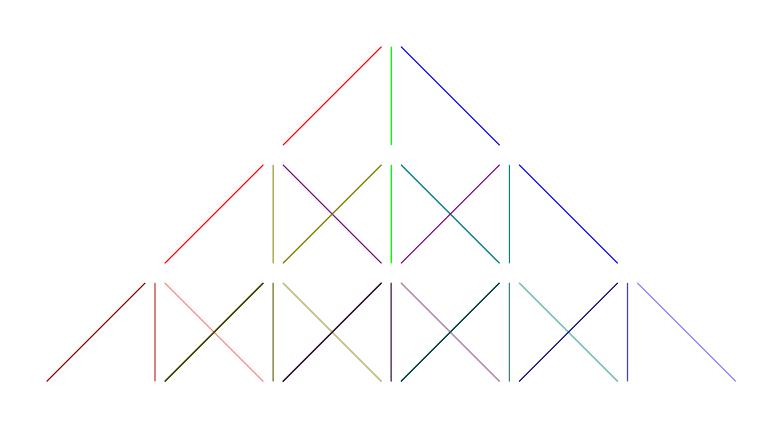
\begin{tikzpicture}

  \node {} child [color=\A] foreach \A in {red,green,blue}
      {
        node {} child [color=\A!50!\B] foreach \B in {red,green,blue}
        {
          node {} child [color=\A!50!\B!50!\C] foreach \C in {black,gray,white}
          {
            node {}
          }
        }
      };
\end{tikzpicture}
\end{document}
